% Design Specifications
\chapter{Design Description}

\section{Wheelchair Storage}

\subsection{The platform}

As explained in the design requirements, our platform had to be able to support the weight of a very heavy power wheelchair while at the same time being as lightweight as possible. For this reason, we decided to make the main parts of our platform out of aluminum. In the future, we can imagine a platform constructed out of composite material that would increase the strength and decrease the weight. However, for our proof of concept, aluminum turned out to be a great material choice. 
 
Indeed, this material is very resistant, it has a yield stress of 240 MPa and it is very light with a density of 2.7 g/cm3. In terms of feasibility, it was also relatively easy to find the aluminum we needed at a reasonable price. We purchased a 0.125in thick flat plate of aluminum with the following dimensions- 36’’x50’’. These dimensions are slightly larger than what is considered to be the minimum amount of area for securing a wheelchair according Federal Motor Vehicle Safety Standard 222. We also ordered 80/20 made to create the structure, reinforce the main frame and make the handle of the platform.
 
\begin{figure}[h]
\centering
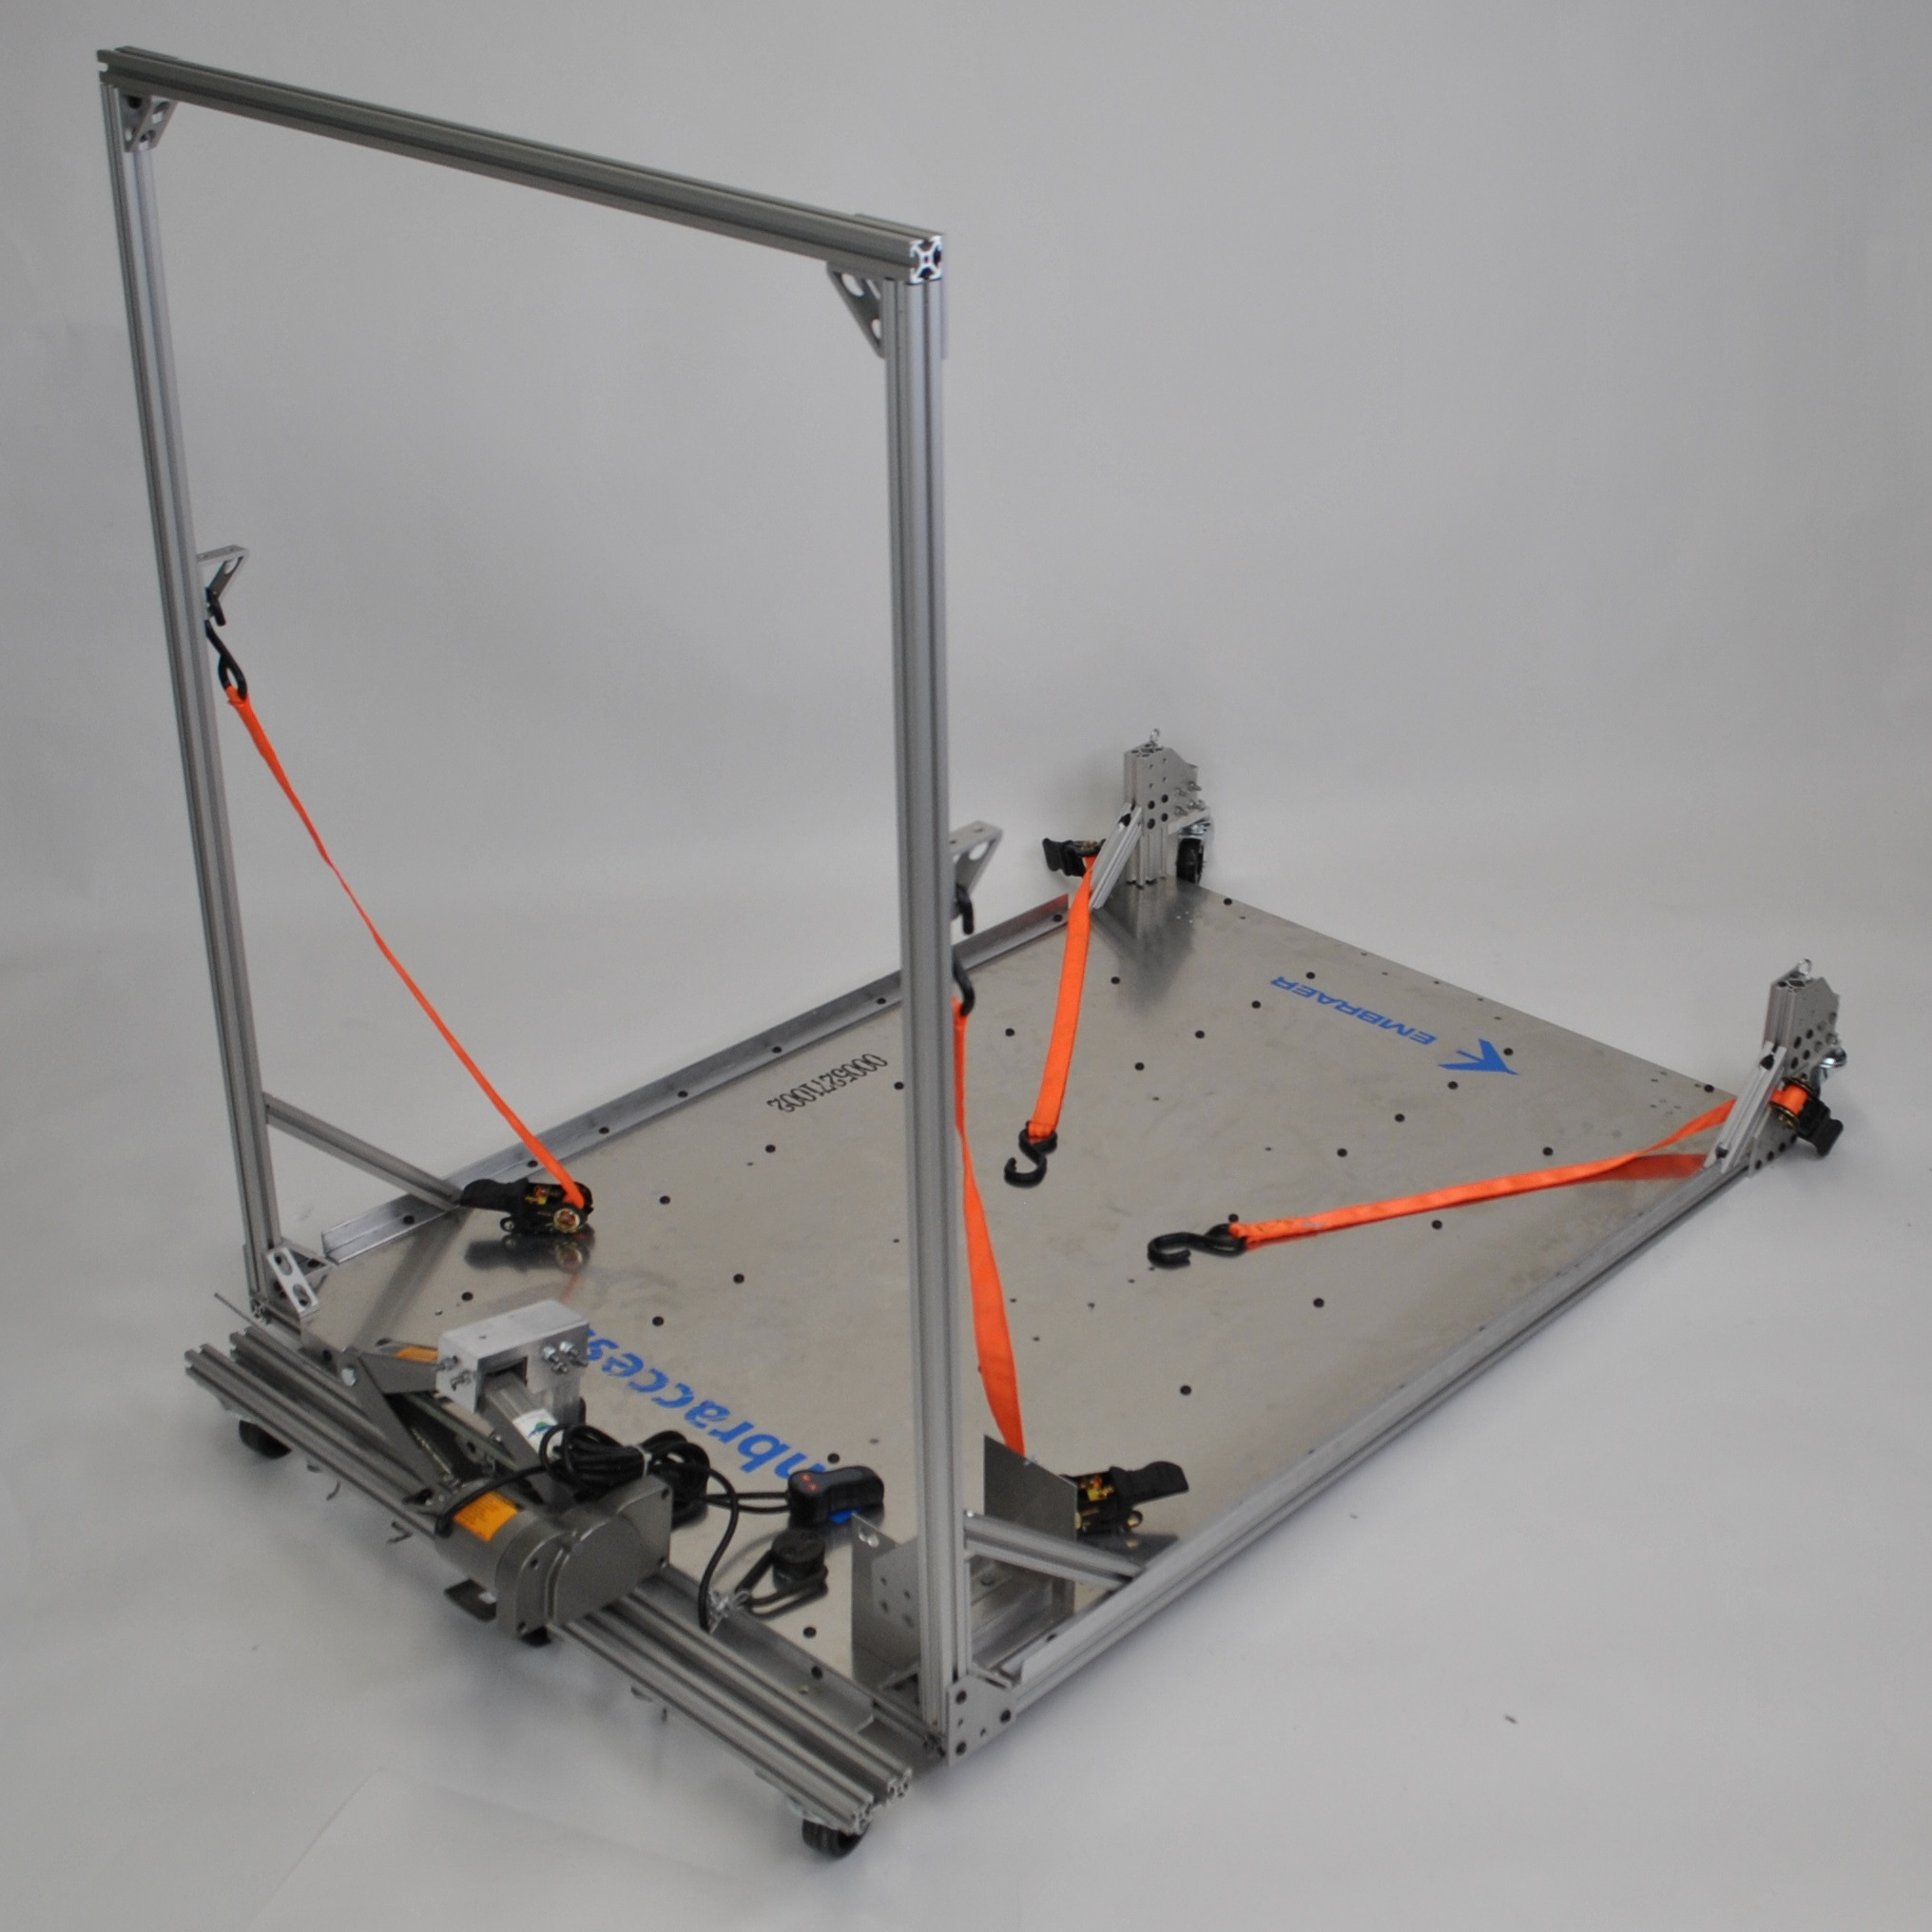
\includegraphics[width=9cm]{images/platform1.jpg}
\caption{The platform we designed using aluminum}
\label{fig:platform1}
\end{figure}
 
As we were analyzing and simulating the effects of the wheelchair load with ANSYS, we realized we needed to add a frame under the aluminum plate because the flat plate would bend if the load applied exceeded 300lbs. As shown in figure \ref{fig:platform2} the ANSYS analysis which was carried out for a 400 pound load applied at four contact points (each one simulating a wheel) shows a lot of bending. The maximum deflection in this case was 2.6 inches, a deflection that is no longer negligible.
 
\begin{figure}[h]
\centering
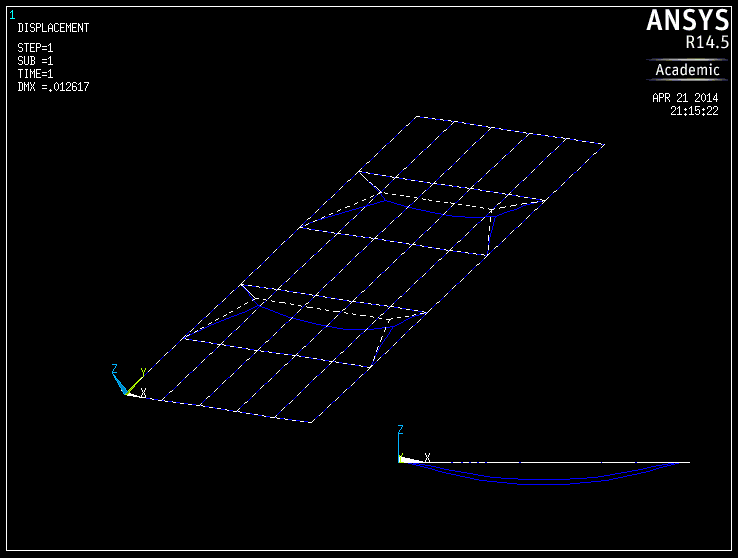
\includegraphics[width=10cm]{images/platform2.png}
\caption{ANSYS analysis of the platform aluminum plate}
\label{fig:platform2}
\end{figure}
 
For this reason, we chose to increase the stiffness of the plate by adding an 80/20 bar along the sides of the platform and three additional 80/20 bars in the middle. This was enough to decrease the bending of the aluminum and did not add much weight (roughly 20 pounds)
 
Because we needed to raise and lower the platform (see moving mechanism section for more details), we decided to add extra stiffness on the edges by adding an aluminum angled bar on each side as shown in figure \ref{fig:platform3}.
 
\begin{figure}[h]
\centering
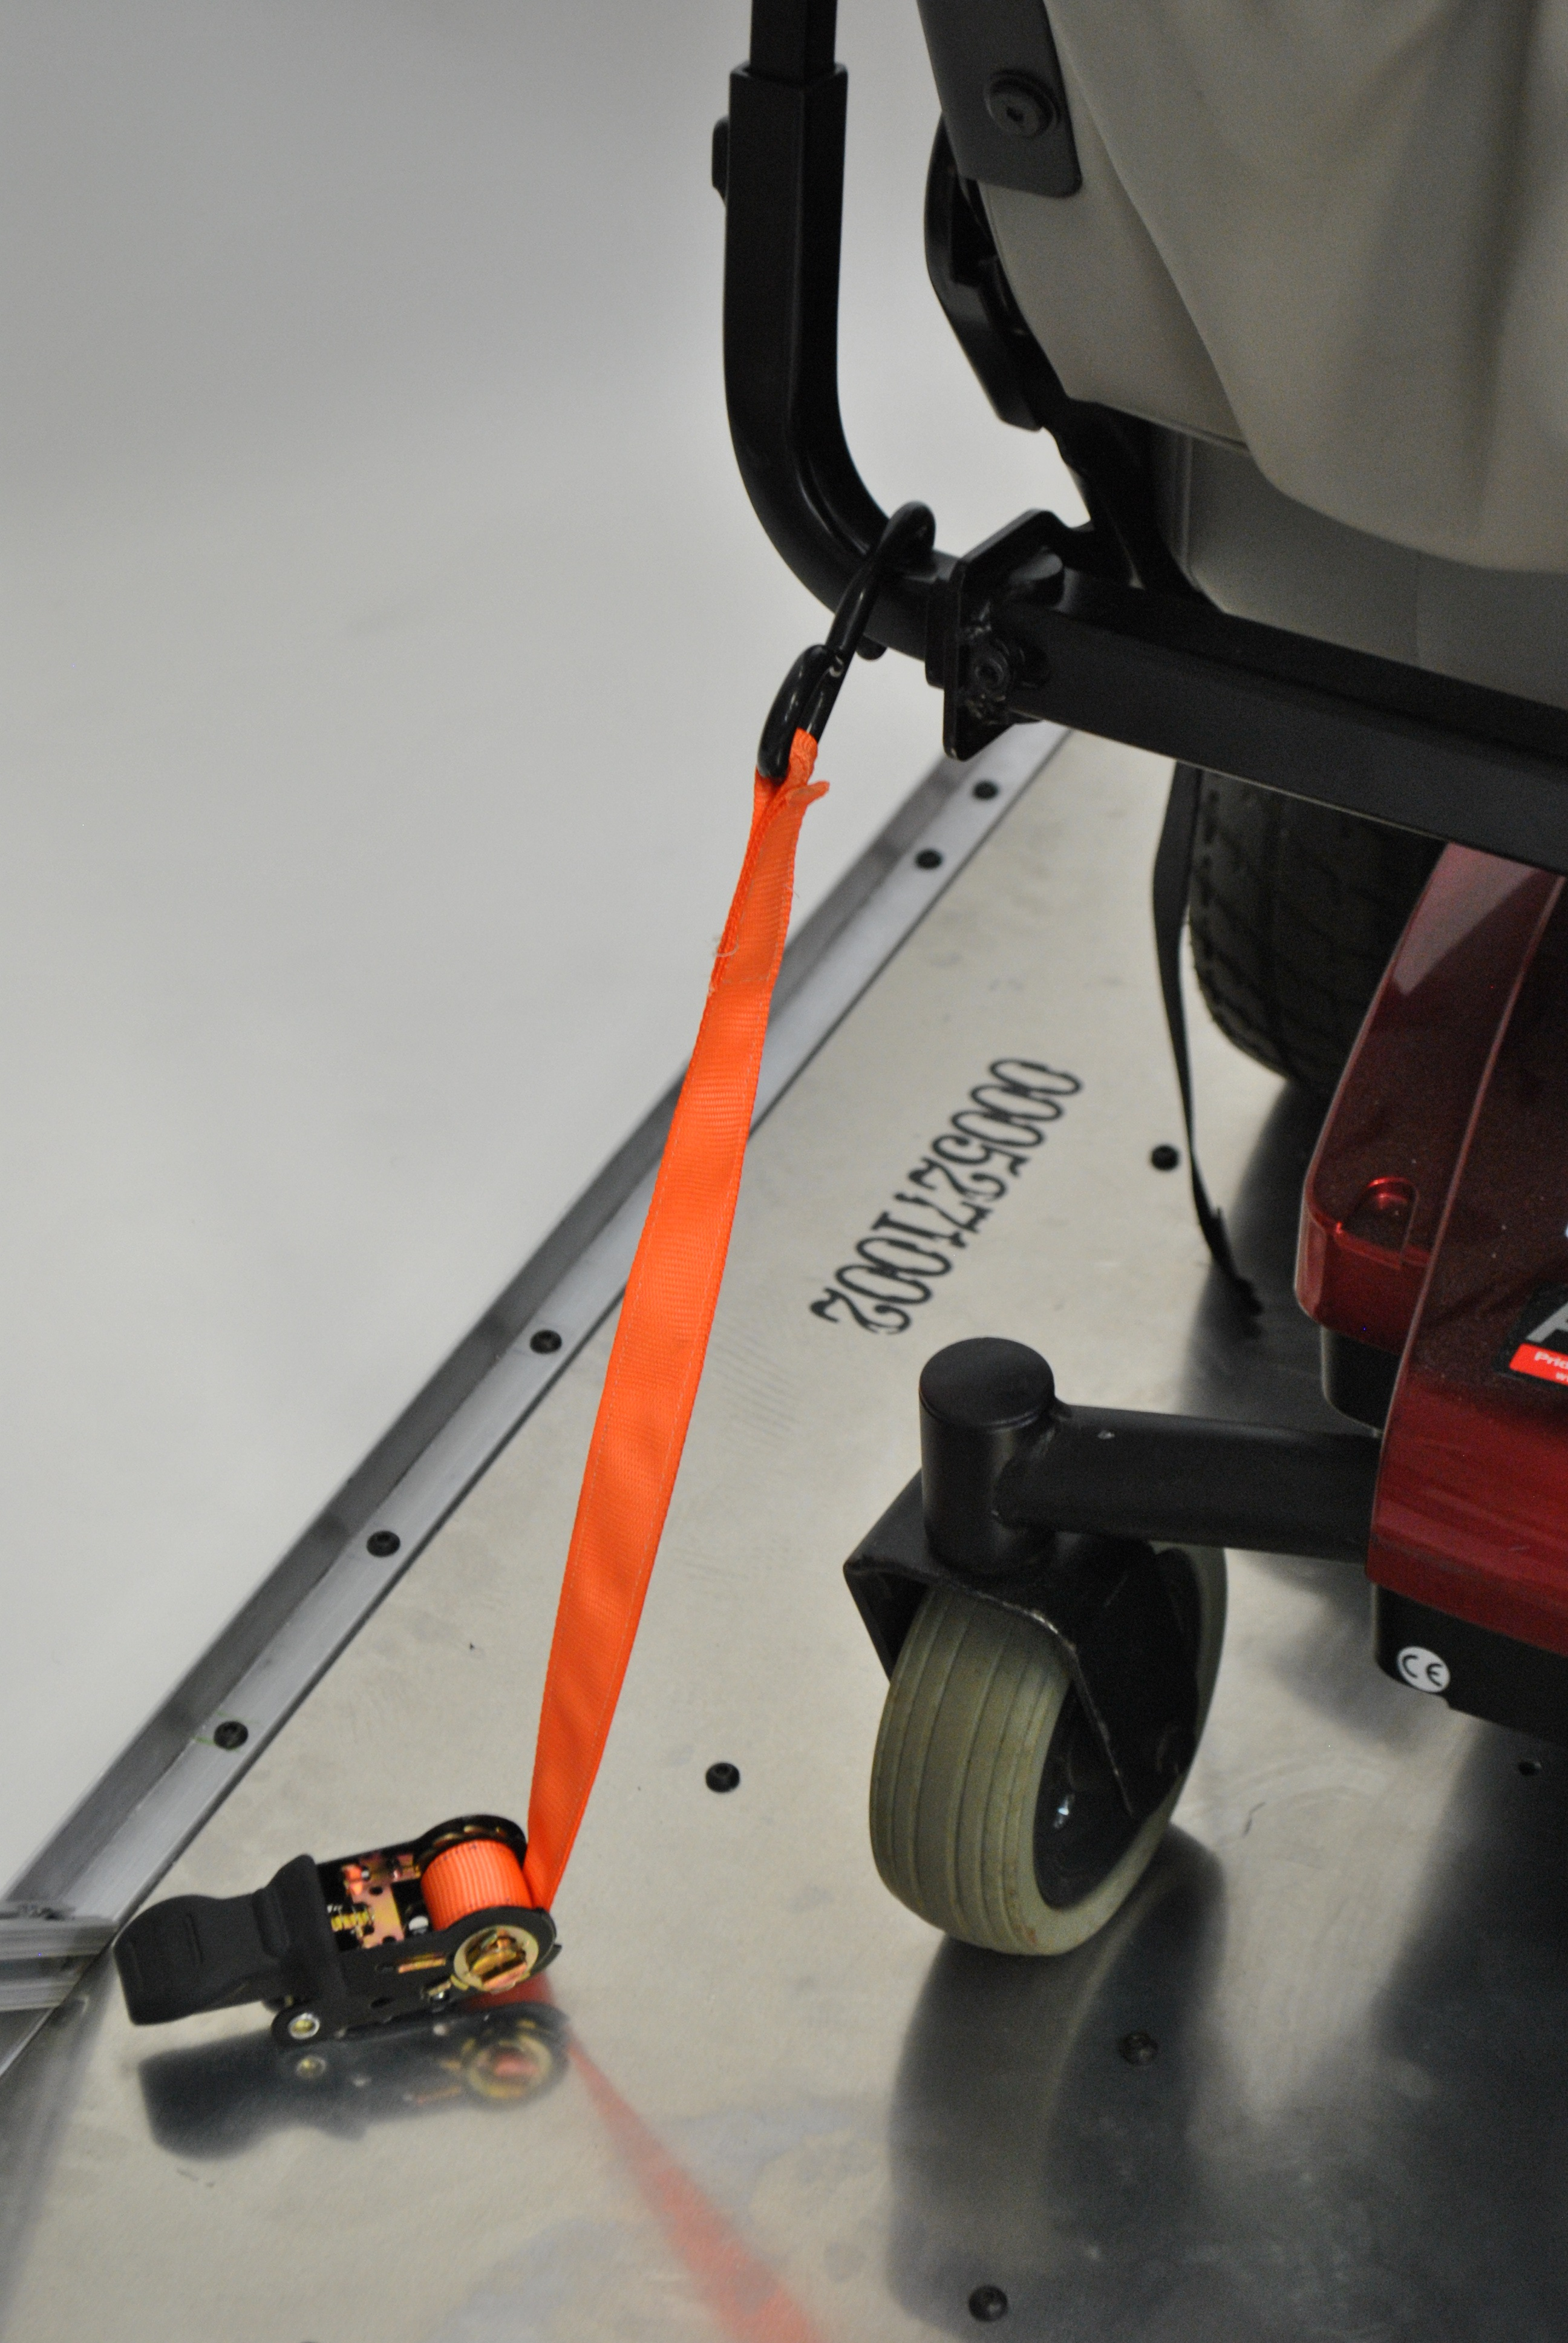
\includegraphics[width=7cm]{images/platform3.jpg}
\caption{The angled bar and the straps we added to the platform}
\label{fig:platform3}
\end{figure}
 
Figure \ref{fig:platform3} also shows another feature we added to the main part of the platform: the straps. As explained previously, we needed to secure the wheelchair once it was on top of the platform. We decided to use straps found in public transportation today because our users are already familiar with them and they trust them. We did not add any other protection device because through our needfinding we were able to infer that wheelchairs mainly get damaged when travelling from the jet way to the cargo hold. Indeed, wheelchairs are the last item put inside the cargo hold and the first one taken out, so it is unlike that baggage handlers throw bags on top of it and airline employees generally use nets inside the cargo hold to make sure heavy items remain static. For this reason, we chose to only use the straps to tie down the wheelchair and did not add other protection device. We could imagine that a next version of our prototype could have inflatable or other material to protect the wheelchair. 
 
The last main feature of the platform is the handle. As you can see from Figure \ref{fig:platform1}, we made it out of the aluminum 80/20. We designed it such that baggage handlers were pushing the platform and not pulling it since this would enable them to look at the wheelchair while moving the whole system. To determine the optimal height of the handle our team did some research on ergonomics of dollies and pallet jack. We found out that according to the Center for Occupational Health and Safety the ideal height was 44 inches from the ground as shown in Figure \ref{fig:platform4}. This is the appropriate placement for an average adult who is 5 feet 8 inches  to use his/her arms to push something heavy while minimizing the effort required to do so. In the future, we could improve the ergonomics of this handle by adding a silicon sleeve to the section that is in contact with handlers’ hands, giving them further information on where exactly they should push and providing them with a more comfortable way to do so.

\subsection{The moving mechanism}

\subsection{The electronics}





\section{Embraccess Aisle Wheelchair}

Users today suffer as they have to perform uncomfortable and unsafe transfers between their wheelchair, the aisle wheelchair and the airplane seat (e.g. while boarding or disembarking, or to use the restroom). Redesigning the accessibility of an airplane is therefore critical to improving the overall experience for wheelchair users. By doing this, both airlines and airplane manufacturers can improve their brand image and profitability by reassuring the company's commitment to social values, by reducing the time spent on the ground and by gaining entry to new markets.

By focusing on the enhancement of the current aisle wheelchair, we developed a product that improves the users independence, comfort and safety. Furthermore, it benefits those who handle the aisle chair by reducing the time and effort spent during transfers.

The following sections explain in detail the design of the Embraccess Aisle Wheelchair:

\subsection{The Big Picture}

The Embraccess Aisle Wheelchair is unique because of its innovative front rest and sliding mechanism that allows users to be supported by and to rest comfortably on the chair and transfer easily from their wheelchair to the aisle wheelchair and finally to an adapted airplane seat. The main parts of this product are shown in Figure \ref{fig:wheelchair}. 

\begin{figure}[h]
\centering
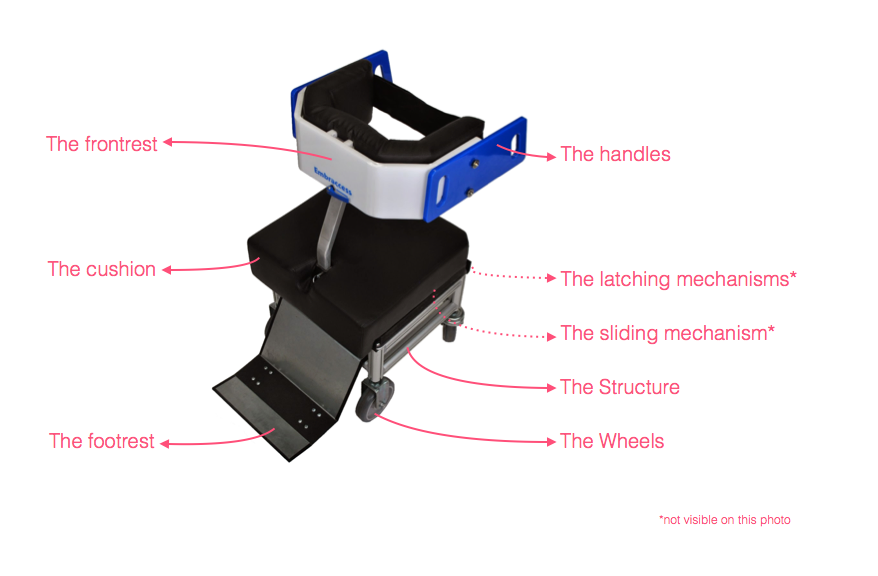
\includegraphics[width=13cm]{images/AisleWheelchair1.png}
\caption{The Embraccess Aisle Wheelchair}
\label{fig:wheelchair}
\end{figure}


\subsection{The Cushion}

The cushion used in this product was especially designed for wheelchair users to provide them the support they need for sitting during prolonged periods of time (i.e.the  flight's duration). It contains a high density flame retardant foam, coated with synthetic leather, that provides both comfort and meets the airplane’s safety requirements. For the next generation of this wheelchair, we recommend substituting this cushion with an air cushion which can provide a higher level of adjustable pressure relief by constantly shifting to the user's body movement.

\subsection{The Structure}
Aluminum was chosen as the main material used in wheelchair’s  structure.This is because aluminum provides the structure the product needs without substantially increasing the weight. Rounded aluminum profiles were used to make the base of the chair, while a thin sheet of aluminum was used to provide a plain surface for the transfer casters to slide on.



\subsection{The Wheels}
In order to minimize weight and ease the movement of the wheelchair, two 6" lockable polyurethane swivel caster wheels were used on the rear part of the wheelchair and two 6" fixed caster wheels were used on the front. This arrangement of the casters allows the wheelchair to be locked by the flight attendant and also guarantees maneuverability in confined spaces.




\subsection{The Footrest}

The footrest, shown in Figure \ref{fig:footrest},  is made up of by a thin bent aluminum sheet attached to two 2" swivel caster wheels that provide the user comfort and safety while transferring through the aisle. The angle of the footrest and the rough adherent surface guarantee that the user's feet do not slip off, providing comfort and security to them.
 

\begin{figure}[h]
\centering
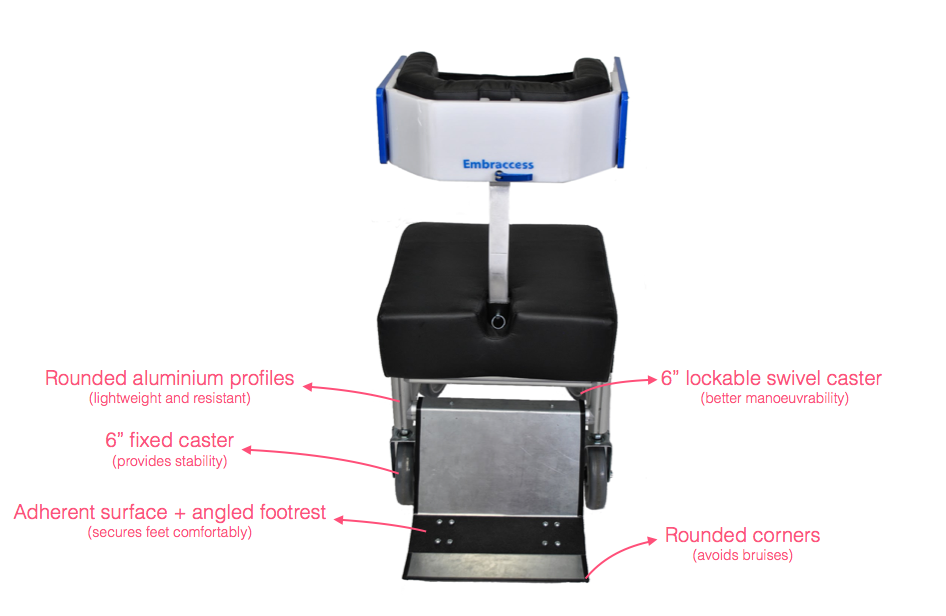
\includegraphics[width=13cm]{images/AisleWheelchair2.png}
\caption{The footrest}
\label{fig:footrest}
\end{figure}

\subsection{The Sliding Mechanism}

The sliding mechanism, shown in Figure \ref{fig:sliding},  consists of .35in diameter spheres positioned under a wooden base that supports both the cushion and the frontrest housing. The equidistant position of the spheres under the base were defined to allow a smooth transfer and  guarantee the contact of the spheres at all times during the transfer. A gap of up to 3.1in may be overcome because of the positioning of the casters. For the next generation of this aisle chair, we suggest that the base should consist of a different material such as aeronautical aluminium to optimize the weight of the mechanism as a whole.

\begin{figure}[h]
\centering
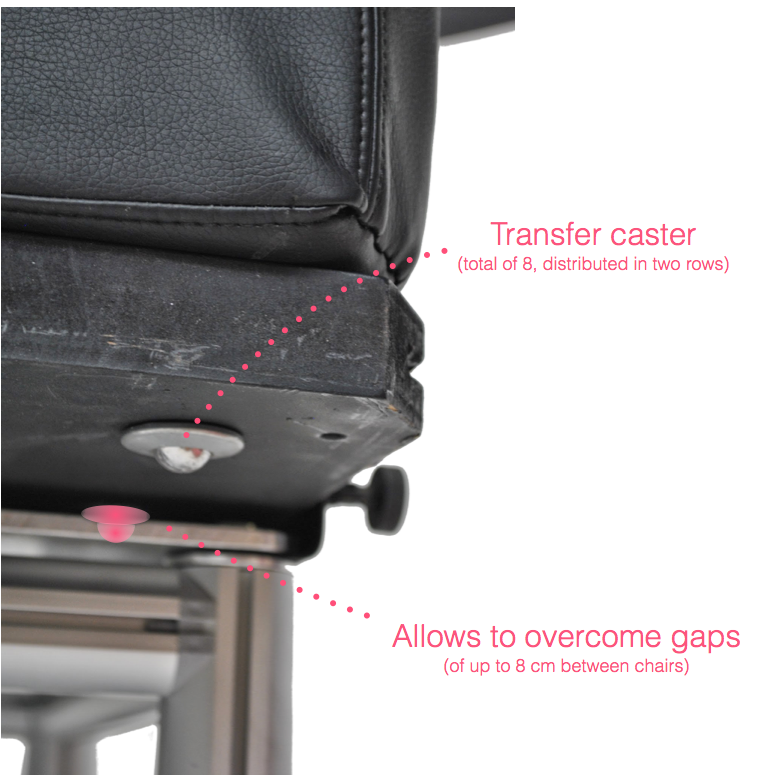
\includegraphics[width=9cm]{images/AisleWheelchair3.png}
\caption{The sliding mechanism}
\label{fig:sliding}
\end{figure}

\subsection{The Latching Mechanism}

The latching mechanisms were developed to allow for an intuitive and safe design. One of the module, show in Figure \ref{fig:latching},  consists of two pins, one at each side of the sliding base that prevents the cushion from sliding laterally. To unlock the latching mechanism, one simply has to pull and turn the pin that is closer to the airplane seat. The other module consists of two static aluminum profiles, located in front and behind the cushion base, that guarantee that the chair does not move forward or backward independently of the rest of the chair. Lastly, a removable pin locks the frontrest to the sliding base as can be seen in Figure \ref{fig:base}.
	For the next generation of this aisle wheelchair, we suggest that the sliding latching mechanism should be linked to a mechanism that detects when both aisle wheelchair and airplane seat are properly aligned, thus improving the transfer and the user's sense of independence.

\begin{figure}[h]
\centering
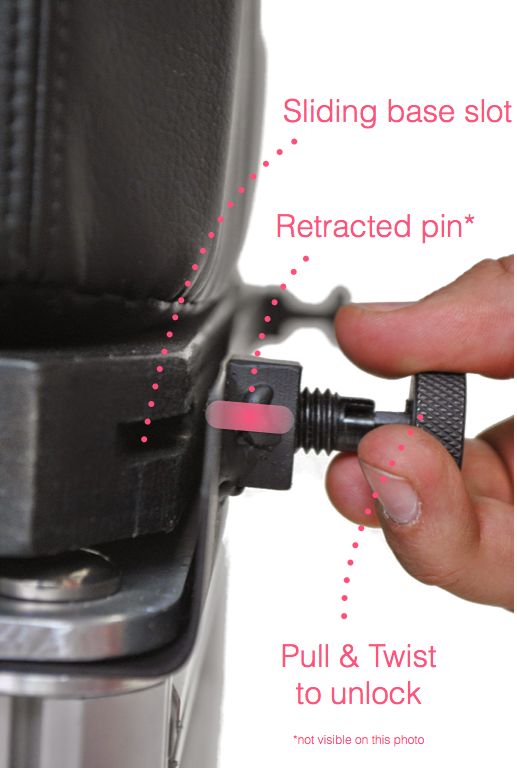
\includegraphics[width=5cm]{images/AisleWheelchair4.png}
\caption{A close up of the latching mechanism}
\label{fig:latching}
\end{figure}


\begin{figure}[h]
\centering
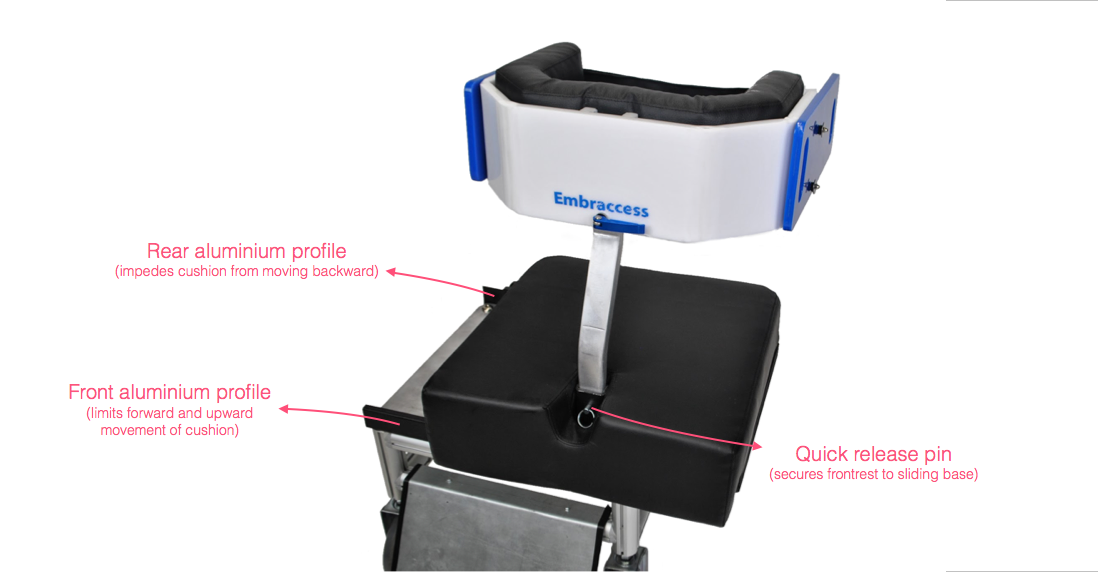
\includegraphics[width=13cm]{images/AisleWheelchair5.png}
\caption{Diagram of whole latching mechanism}
\label{fig:base}
\end{figure}

\subsection{The Frontrest (Chestrest)}
The frontrest, shown in Figure \ref{fig:frontrest},  was conceived so that it would provide support for the user while he is being laterally transferred. Its unique design allows the user to make a frontal transfer from his wheelchair to the aisle wheelchair and perhaps a backward transfer from the aisle wheelchair to the airplane's toilet seat (this still has to be tested). The U-Shaped support combined with the cushion and back strap provide the users with increased support and comfort, allowing them to move around the aisle and make lateral transfers easily and safely. The quick release latch located right below the Embraccess logo allows for the height of the front rest to be adjusted, making it flexible for different types of users. Furthermore, the rigid mast made of aluminum securely attaches the front rest to the sliding cushion base. Lastly, the vertical and horizontal slots on the U-Shaped Support allows the handles to be adjusted (see "The Handles" for more details).

\begin{figure}[h]
\centering
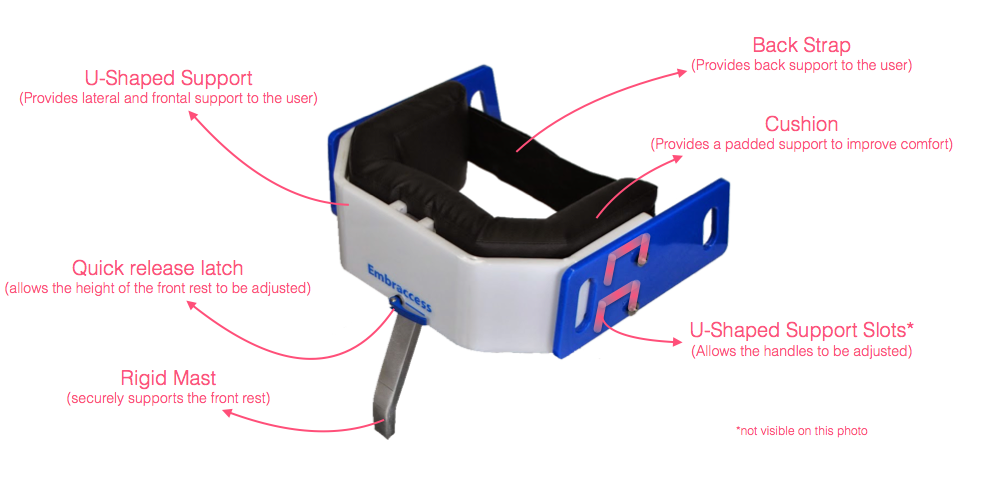
\includegraphics[width=13cm]{images/AisleWheelchair6.png}
\caption{Diagram of the Frontrest}
\label{fig:frontrest}
\end{figure}

\subsection{The Handles}
The handles, shown in Figure \ref{fig:handles}, are made of two acrylic parts that can be adjusted to allow the people maneuvering the wheelchair to pull or push it from both the rear and front of the aisle wheelchair. This is extremely important in confined spaces like airplanes because one cannot reach the other side of the wheelchair. In the future,  the handles would be made of  lighter materials. Nevertheless due to budget and fabrication limitations, this heavier plastic was used.


\begin{figure}[h]
\centering
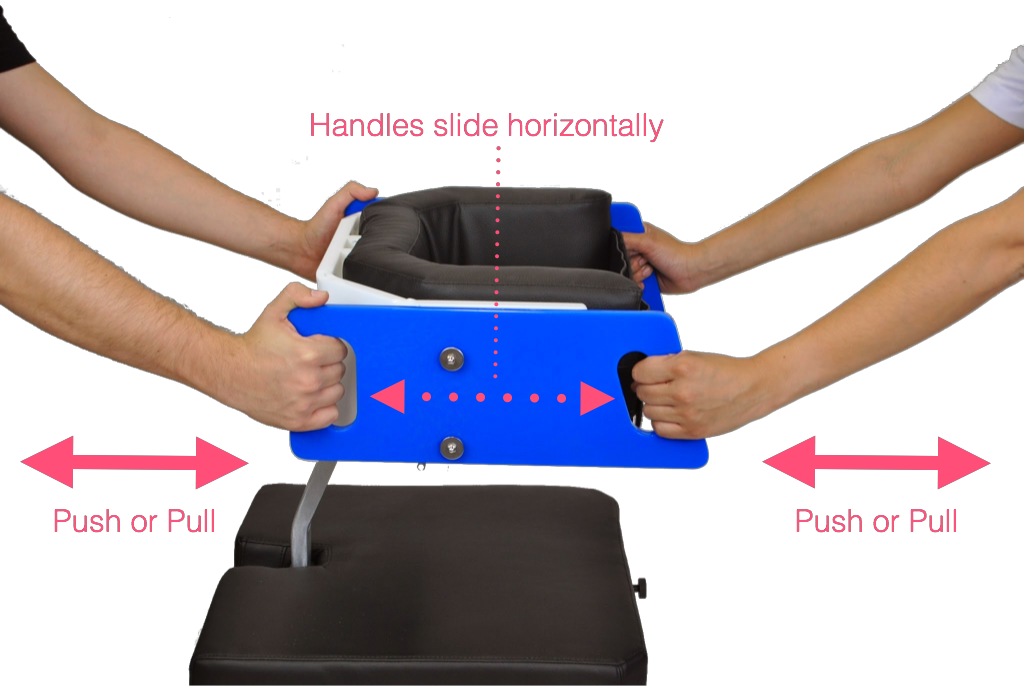
\includegraphics[width=9cm]{images/AisleWheelchair7.png}
\caption{The adjustable handles}
\label{fig:handles}
\end{figure}

\subsection{The Optional Seat Belt}
An optional seat belt was added to our design that securely maintains the user's legs positioned away from obstacles while being transferred through the aisle. This seatbelt is only required for users whose legs spread involuntarily.

\subsection{Others}
\textbf{The Beasy Board}
	This transfer board shown in Figure  \ref{fig:board} eases the frontal/backward transfer between the user's wheelchair and the aisle wheelchair by reducing the friction and eliminating the gap between the two chairs.

\begin{figure}[h]
\centering
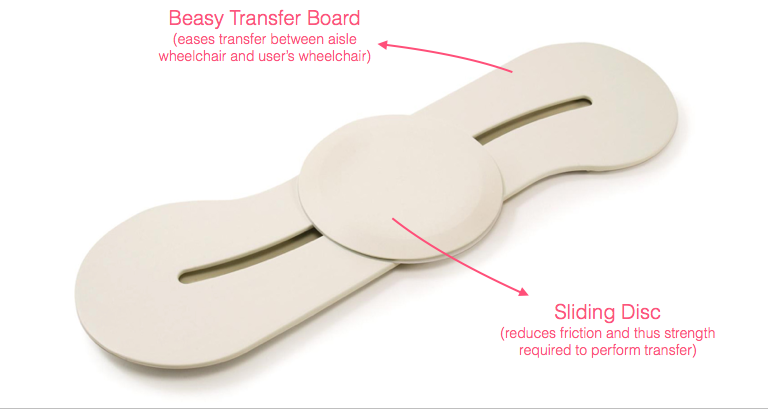
\includegraphics[width=10cm]{images/AisleWheelchair8.png}
\caption{The Beasy Board}
\label{fig:board}
\end{figure}

\textbf{The Airplane Seat}
	A simple adaptation of the airplane's seat, shown in Figure \ref{fig:airplane}, was made in order to demonstrate the concept of our project. A redesigned aisle seat would be required in order to make the Embraccess Aisle Wheelchair work flawlessly, as it requires a planar surface for the casters to slide and retractable armrests that do not obstruct the transfer path.

\begin{figure}[h]
\centering
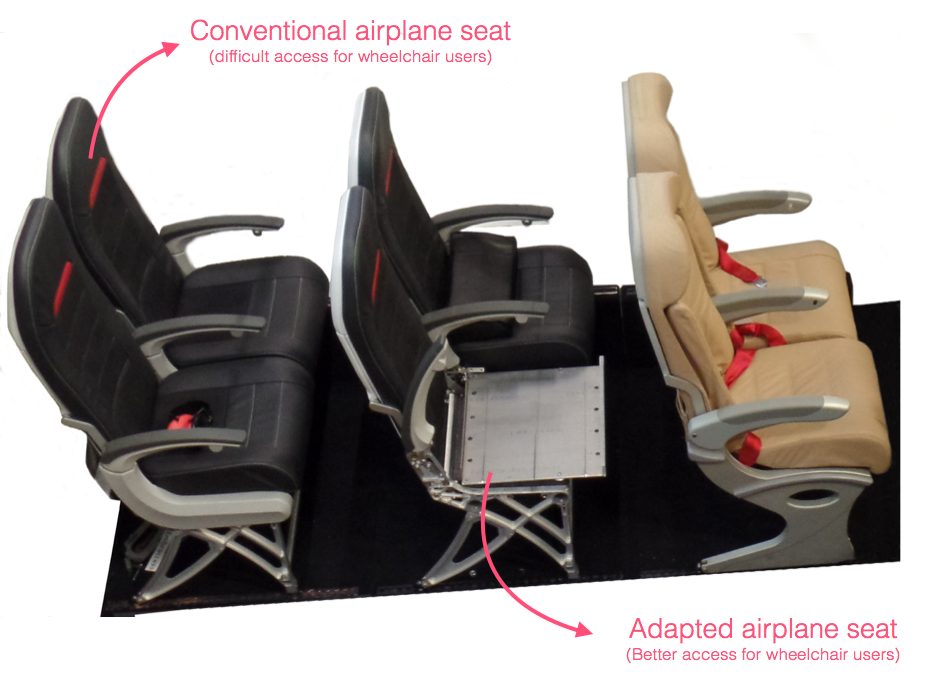
\includegraphics[width=10cm]{images/AisleWheelchair9.png}
\caption{The Airplane Seat}
\label{fig:airplane}
\end{figure}

\newpage

\section{User feedback about the whole experience}


